\documentclass{book}
\usepackage[left=2cm,right=2cm, top=2cm,bottom=2cm,bindingoffset=0cm]{geometry}
\usepackage[utf8]{inputenc}
\usepackage[russian]{babel}
\usepackage[OT1]{fontenc}
\usepackage[dvips]{graphicx}
\graphicspath{{images/}}
\usepackage{amsmath}
\usepackage{amsfonts}
\usepackage{amssymb}
\title{Алгоритм "Spigot" для нахождения числа $\pi$}
\date{}
\begin{document}
\maketitle
\paragraph{Общее описание. Преимущества. Недостатки.\\}
\begin{normalsize}
Алгоритм основан на представлении чисел в смешанной системе счисления. Некоторые иррациональные числа становятся периодическими в таких системах. Подробное описание этого приводится ниже. Основным преимуществом алгоритма является то, что он использует только целочисленную арифметику для получения каждого знака. Вероятно, поэтому авторы алгоритма пназвали его именно так (spigot англ. "кран"). Каждое число вытекает, подобно каплям из "крана". Также к преимуществам можно отнести еще размер программы. Основным недостатком является то, что диапазон работы алгоритма ограничен памятью, но для данной задачи этот недостаток не проявляется. Итак, чтобы понять принцип работы алгоритма, разберём более простой пример.
\end{normalsize}
\paragraph{Система счисления в которой знаки числа $e$ периодические.\\}
\begin{normalsize}
Простейшим примером смешанной системы счисления является дата. Т.е d дней, h часов, m минут, s секунд будут представлены как $d \cdot 24 \cdot 60 \cdot 60 + h \cdot 60 \cdot 60 + m \cdot 60 + s$ секунд.\\
Теперь ближе к делу. Как хорошо известно, число можно представить в виде многочлена. Например,\\
$$\sqrt{2} = 1.41421356... = 1 + \frac{1}{10}(4+\frac{1}{10}(1+\frac{1}{10}(4+\frac{1}{10}(2+\frac{1}{10}(1+...))))$$
Т.е. сейчас мы имеем представление числа в системе $(\frac{1}{10}, \frac{1}{10}, \frac{1}{10}, ...)$. Теперь если мы сменим это представление на представление в системе $\textbf{b}=(\frac{1}{2}, \frac{1}{3}, \frac{1}{4}, \frac{1}{5}, ...)$. Тогда имеем представление корня из 2.
$$a_0 + \frac{1}{2}(a_1+\frac{1}{3}(a_2+\frac{1}{4}(a_3+\frac{1}{5}(a_4+\frac{1}{6}(a_5+...))))$$
Где  $a_i$ неотрицательные целые числа. Если $0 <= a_i <= i$ для $i >= 1$, то представление называется регулярным. В такой системе число имеет вид $(a_0,a_1,a_2,...)_{\textbf{b}}$. Каждому числу сопоставляется такое представление. При этом имеет место важное замечание. Мы исключаем представления, которые заканчиваются максимальными знаками. Т.е, например, $\frac{1}{2} = (0,1,0,0,...)_{\textbf{b}} = (0,0,2,3,4,5,6,...)_{\textbf{b}}$. Первое представление мы исключаем.
\end{normalsize}
\subparagraph*{Лемма 1.(без доказательства)\\}
\begin{normalsize}
		(a) Если $i >= 1$, $(0,0,0,...,0,a_i,a_{i+1},...)$, $b < \frac{1}{i!}$, в частности, $(0,a_1,a_2,a_3,a_4,...)_b < 1$.\\
		(b) Представления чисел использующие систему $b$ единственные.\\
		(c) Целая часть $(a_0,a_1,a_2,a_3,a_4,...)_b$ $a_0$, а дробная $(0; a_1, a_2, a_3, a_4, ...)$\\\\
\end{normalsize}
\begin{normalsize}
В этой системе, некоторые иррациональные числа становятся периодическими. Например, число $e = (2; 1, 1, 1, ...)_b;$ (это просто иная запись ряда $\sum \frac{1}{i!}$)\\
$$1+\frac{1}{1}(1+\frac{1}{2}(1+\frac{1}{3}(1+\frac{1}{4}(1+\frac{1}{5}(1 + ...))))).$$
Десятичные знаки вещественного числа x, могут быть получены взятием целой части от x, умножения его дробной части на 10, взятия целой части числа, умножения дробной части и т.д. Если $x = (a_0;a_1,a_2,...,a_n)_{\textbf{b}}$, тогда $10x = (10a_0;10a_1,10a_2, ... , 10a_n)$. Для того, чтобы привести полученное число к регулярному виду, будем уменьшать $i$-е число по модулю $i$. Начиная эти сокращения справа, перетаскиваем полученные частные влево и так до 0-ого элемента (последнее частное и будет являться искомым знаком). Таким образом получим регулярное представление числа $10x$ в этой системе. и так далее, опять домножим текущее представление на 10, затем полученное снова домножим на 10... Демонстрация для первых трех чисел приведена в таблице ниже.
\begin{figure}[h!]
\center{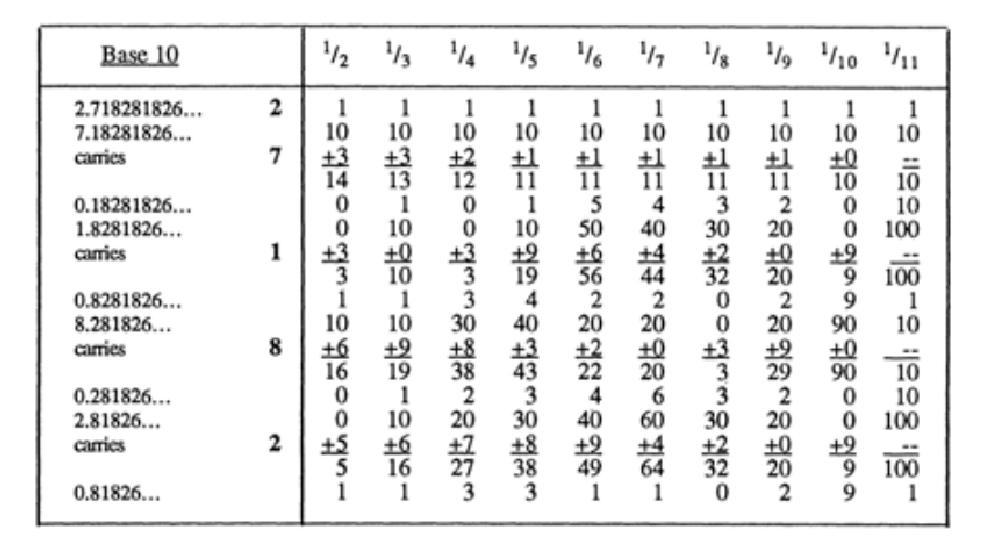
\includegraphics[]{1}}
\caption{Здесь жирным выделены знаки числа e. Сокращения выполняются по модулю $i$. Первый знак результат аппроксимации.}
\end{figure}
\end{normalsize}
\paragraph{"Spigot" для знаков числа $\pi$.}
\begin{normalsize}
Для числа $\pi$ можно провести подобные рассуждения (с некоторыми отличиями). Отправной точкой здесь будет являться следующий ряд:\\
$$\pi = \sum_{i=0}^{\infty} \frac{(i!)^{2}2^{i+1}}{(2i+1)!}$$
Который может быть получен из формулы Валлиса для $\pi$. Если этот ряд немного преобразовать, то можно получить, что:\\
$$\frac{\pi}{2} = \sum_{i=0}^{\infty} \frac{i!}{(2i+1)!!} = 1 + \frac{1}{3} + \frac{1 \cdot 2}{3 \cdot 5} + \frac{1 \cdot 2 \cdot 3}{3 \cdot 5 \cdot 7} + ...$$
Что также можно представить в виде:\\
$$\frac{\pi}{2} = 1 + \frac{1}{3}(1 + \frac{2}{5}(1+\frac{3}{7}(1+\frac{4}{9}(1 + ...))))$$
Таким образом получаем новую смешанную систему счисления $\textbf{c} = (\frac{1}{3}, \frac{2}{5}, \frac{3}{7}, \frac{4}{9}, ...)$, в которой $\pi$ представляется в виде $(2,2,2,2,...)_{\textbf{c}}$. Для того, чтобы представление было регулярным, необходимо, чтобы знак на $i$-ом месте лежал в отрезке $[0,2i]$. К сожалению, это еще не все.
\end{normalsize}
\subparagraph*{Лемма 2. (без доказательства)\\}
\begin{normalsize}
Представление $(0,2,4,6,8,...)_{\textbf{c}} = 2$. Следовательно регулярные представления вида $(0,a,b,c,...)_{c}$ лежат в пределах 0 и 2.\\\\
\end{normalsize}
\begin{normalsize}
Лемма 2 означает, что представления в $\textbf{c}$ не единственны. К примеру, $(0;2,4,6,8,...)_{\textbf{c}} = 2 - \frac{2}{3} = \frac{4}{3}$, в то время как $(0;0,2,3,4,...)_{\textbf{c}} = \frac{2}{3} = (0;2,0,0,0,...)_{\textbf{c}}$.\\
Целая часть $(a_0;a_1,a_2,...)_{\textbf{c}}$ может быть $a_0$ или $a_0+1$, в зависимости от того $(0;a_1,a_2,...)_{\textbf{c}}$ принадлежит $[0,1)$ или $[1,2)$. Речь идет о тех ситуациях, когда знак числа $\pi$ получается равным 10, в таком случае на $i$-ом месте, конечно, будет стоять 0, но необходимо и увеличить на единицу предшествующие знаки, а если предшествующий знак был равен 9, то и на его место вписать 0. Продолжать это действие до того, пока не встретится отличный от 9 знак. Теперь можно смело написать алгоритм.\\
\end{normalsize}
\subparagraph*{Алгоритм. $\pi$-spigot.\\}
\begin{normalsize}
	\begin{list}{•}{}
		\item \textit{Инициализация:} Массив остатков remainders = $(2,2,2,...,2)$ (размер массива $[10n/3]$, можно доказать, что этого достаточно)\\
		\item Повторить n раз:\\
		\textit{Умножить на 10}: умножить каждое число в remainders на 10.\\
		\textit{Привести remainders к регулярному виду}: на i-ом месте вычисляем частное (quotient) при делении (remainders[i]+ перенос с предыдущего разряда) на $2i-1$ (см. \textbf{c}), вычисляем остаток от деления этой суммы. Оставляем остаток в remainders[i]. Для вычисления переноса умножаем частное (quotient) на $(i-1)$ (числитель соответствующей дроби в $\textbf{c}$).\\
		\item Далее если частное получилось равным 10, то в res[i] пишем 0, а знак до него увеличиваем на 1, если этот знак равен 9, то тогда пишем и на это место 0, продолжаем пока не встретим знак отличный от 9.
	\end{list}
\end{normalsize}
Нахождение первых знаков числа $\pi$ проиллюстрировано в таблице ниже.\\
\begin{figure}[h!]
\center{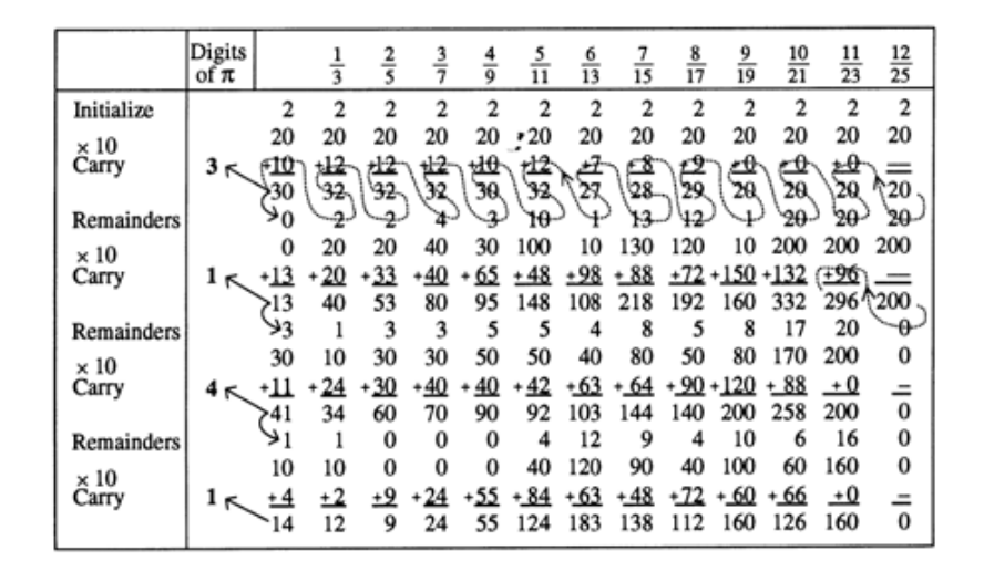
\includegraphics[]{2}}
\caption{Нахождение первых четырёх знаков}
\label{ris:2}
\end{figure}
\paragraph{Возможные улучшения.\\}
Алгоритм можно ускорить благодаря, выводу более, чем по одному знаку за итерацию, однако, тогда необходимо также увеличивать еще и размер выделяемой памяти. Более того, если взять основание, например, 100000, то можно получить удивительно короткую программу (что-то около 15-ти строчек), если быть уверенным, что пределы вычислений в которых будет работать программа не содержит комбинации знаков 00000.
\end{document}